\chapter{Literature Review}
Hypernymy identification and discovery are broadly split into pattern-based and distributional methods \citep{camacho2018semeval, Wang2017}.  The two classes need not be mutually exclusive and we will encounter hybrid methods which integrate features from both approaches, improving on the result achieved by employing each respective method independently  \citep{shwartz2016path, bernier2018crim}.  Despite being overshadowed by distributional methods in recent years, there has been renewed interest in pattern-based methods \citep{roller2018hearst}, a fact that underscores their continued relevance.

\section{Pattern-Based Methods} \label{Pattern-Based Methods}
Lexico-syntactic patterns frequently occurring in language encode the hypernymy semantic relationship between words bound to the patterns.  Such patterns are still referred to as Hearst patterns in tribute to the Marti Hearst's pioneering work on hypernym discovery more than 25 years ago \citep{hearst1992automatic}.

\subsection{Hearst Patterns} \label{Hearst Patterns}
\citeauthor{hearst1992automatic} kick-started the chase for hypernyms when she proposed that the text corpus itself contained information about the language in which it was written \citep{hearst1992automatic}.  She observes that an unknown word within a text can be understood by the reader via word pattern co-occurrences that unambiguously entail the word to a familiar superordinate term \citep{hearst1992automatic}.  Consider the following sentence snippet:

\say{African birds such as turacos, trogons and nicators are…}

The phrasing conveys a semantic \textbf{is-a} relationship between \textit{turacos, trogons and nicators} and the more generic term \textit{bird}.  The compound noun \textit{African bird} is a more specific type of bird and more general than a \textit{turaco} making it a hypernym of \textit{turaco} and hyponym of \textit{bird}.  Anyone reading this excerpt only needs to be familiar with the concept of \textit{bird} to acquire some knowledge of what a \textit{nicator} is.  In the absence of the [Y such as X] syntactic pattern, the sentence contains no other clues on what a \textit{trogon} could mean.  The pattern is also able to expose a co-hyponym relationship between \textit{turacos, trogons and nicators}, all them being a type of bird.  

The variety of free text initially casts doubt on whether representative lexical constructs can be found at all.  Notwithstanding, armed with a few seed examples, Hearst was able to bootstrap a system to automatically acquire six high-quality patterns \citep{hearst1992automatic} from the Grolier’s Academic Encyclopedia digitised corpus \citep{grolier1990academic}:

\begin{itemize}
    \item X [,] and other Y
    \item X [,] or other Y
    \item Y [,] such as X
    \item Y [,] including X
    \item Y [,] especially X
    \item Such Y as X
\end{itemize}

To harvest the patterns, Hearst first collected a list of word-pairs for which the hypernymy relation holds and recorded the textual environment in which the words featured.  High frequency environments were considered predictive of hypernymy and were converted to generalised patterns.  The new patterns were subsequently used to find new seed word-pairs which further fuelled the cycle of pattern discovery \citep{hearst1992automatic}.  Although Hearst focused on English, lexico-syntactic patterns were also induced in a wide variety of languages: Spanish, French, Italian, Dutch \citep{faralli2018misa}; Swedish \citep{rydin2002building} in \citep{sahin2017}; Turkish \citep{sahin2016extraction} in \citep{sahin2017}; and Chinese \citep{Fu2014}.

The pattern-based approach is not necessarily amenable to locate other semantic relations.  Hearst was not able to identify high-yield patterns that identify meronymy \citep{hearst1992automatic}, although more success was observed in languages other than English \citep{sahin2017}.  Hypernymy might be particularly suited to this technique due the classification nature of the relation.  This hypothesis also makes an encyclopedia an ideal corpus from which to extract hypernyms due to the high concentration of definitions within such a text.    This justifies Wikipedia as the corpus of choice in diverse tasks such as taxonomy learning \citep{bordea2016semeval} and linguistic resource construction \citep{Flati2016, Baroni2011}.  

Lexico-syntactic patterns are not entirely resistant to the ambiguity of language.  \citeauthor{wu2012probase} provide several sample phrases where the application of Hearst patterns leads to incorrect hypernyms \citep{wu2012probase}.  \say{Animals other than dogs such as cats…} will result in \(hypernym(cat, dog)\) which is an obvious false positive \citep{wu2012probase}.  Consequently, pattern-based methods sacrifice precision for recall \citep{Wang2017, Snow2004, ritter2009anyway}.  This is exacerbated by the constraint that hyponyms must co-occur with their hypernyms within the scope of a sentence which is not always the case in general-purpose texts.  In the SemEval 2018 Shared Task 9 \citep{camacho2018semeval} English general-purpose corpus, most of the training pairs do not even feature in the same paragraph, much less in the same sentence \citep{bernier2018crim}.


Despite these limitations, Hearst’s early attempt yielded results promising enough to inspire related work.  7,067 sentences contained the construct \textit{such as} contiguously out of the 8.6-million word corpus \citep{grolier1990academic}.  Within these sentences, 152 hypernymy relations were found that adhered to the experiment’s constraints, chiefly that hypernym and hyponymy terms were unmodified.  Similar to later research \citep{kozareva2010semi}, Hearst compares the results of her pattern-mining algorithm with the noun hierarchy featured in an early version of WordNet (1.1) \citep{Miller1995}, which at the time comprised 34,000 noun forms organised into approximately 26,000 \ac{synset}s.  Of the 152 relations, both words in the hyponym/hypernym word-pair were found in WordNet in 106 cases.  61 of these relations were also found to exist in WordNet.  

Fittingly, Hearst was also the first to observe limitations to her approach.  Some mined hypernyms were overly generic (ex. the hypernym \textit{species} does not convey much about the hyponym other than it is a living organism).  In other cases, the context influenced the hypernym to make it too specific; for instance \textit{aircraft} was found to be a \textit{target} because of the military sense of the text in question \citep{hearst1992automatic}.

\subsection{Extending Hearst with Probabilistic Methods}
The examination of the pattern-based methods’ weaknesses was extended by \citeauthor{Wang2017} who note that the absence of “world knowledge” limited the precision of these methods \citep{Wang2017}.   They present other challenges inherent in Hearst Pattern parsing:
\begin{itemize}
    \item Since hypernym and hyponym words are nouns or noun phrases, several named entities will be excluded since they are not considered noun phrases.  For instance: \say{…classic movies such as Gone with the Wind…} where \textit{Gone with the Wind} is actually a proper noun and type of movie (as well as classic movie);
    \item Named entities sometime feature the word \textit{and} in their name.  Examples include \textit{Proctor \textbf{and} Gamble}, \textit{Alf Mizzi \textbf{and} Sons Ltd.}, \textit{Plough \textbf{and} Anchor} etc. A pattern like \say{…companies such as IBM, Nokia, Proctor and Gamble…} will consider \textit{Proctor} and \textit{Gamble} to be two different hyponym candidates;
    \item Co-hyponym lists can contain mixed types.  For example: \say{…representatives in N America, Europe, the Middle East, Australia, Mexico, Brazil, Japan, China, and other countries…} features a mix of continents/regions and actual countries.  A literal interpretation of this pattern would result in \(hypernym(Europe, country)\) which is clearly wrong;
\end{itemize}

\citeauthor{Wang2017} mitigate the ambiguity inherent in pattern-mining by proposing an unsupervised, iterative process that refines the collection of harvested hypernym pairs together with a knowledge dictionary over several epochs, designed to improve both precision and recall \citep{Wang2017}.  The process is broken down into three sub-procedures.  

The Hearst-like patterns are first applied on each sentence of an input corpus text.  Given that they adhere to some imposed constraints, noun phrases are added to a list of potential hypernyms and hyponyms respectively.  All combinations of compound noun phrases such as \textit{Proctor and Gamble} are considered (i.e. \textit{Proctor}, \textit{Gamble}, and \textit{Proctor and Gamble}).  This step generates a list of subordinate words and a list of potential hypernyms for every parsed sentence.  The latter list needs to be reduced to the single, most likely hypernym \citep{Wang2017}.

In the second sub-procedure, conditional probability is used to choose the most likely hypernym from two or more potential superordinate words mined from a single sentence.  The algorithm measures the probability of each candidate word being a hypernym of the collected hyponyms by referring to the knowledge dictionary.  Note that the knowledge dictionary contains high confidence word-hypernym pairs.  The word recording the highest conditional probability $p(y_i | X_s)$, where $y_i$ $\in$ $\{y_1,\ldots,y_n\}$ are candidate hypernyms and $X_s=\{x_1,\ldots, x_m\}$ are collected hyponyms, is chosen as the most likely hypernym in the sentence.  The co-hyponyms in \(X_s\) are assumed to be independent and equally related to the hypernym \citep{wu2012probase}.

The third sub-procedure takes on the mined co-hyponym list and estimates the validity of each of the captured hyponyms.  This step is needed to determine whether conjoined noun phrases (ex. \textit{Proctor and Gamble}) represent separate words or should be taken as an atomic entity.  Another objective of this step is to find the longest sequence of conjoined terms in which co-hyponymy applies, given sentences like \say{… representatives in N America, Europe, the Middle East, Mexico, Brazil, Japan and other countries …}.  In the absence of world knowledge, this mix of continents, regions and actual countries could all be considered \textit{country} subordinates based on the pure application of the Hearst pattern.  With the help of the knowledge dictionary, a similar probabilistic mechanism is employed here too, to determine the likelihood of each of these terms co-occurring with other already-discovered terms linked to the \textit{country} hypernym \citep{wu2012probase}.  

The algorithm produces a set of hypernymy relations which make up the edges of a taxonomy.  The construction of the taxonomy itself falls outside the scope of this dissertation although it is worth noting that the probabilistic framework is extended to the taxonomy’s measure of uncertainty with respect to ambiguous information contained within it.  The algorithm was applied on a massive scale:  326 million sentences were extracted from a corpus composed of 1.7 billion web pages to induce 2.7 million distinct concepts; 16.2 million concept-instance pairs and 4.5 million concept-sub-concept pairs \citep{wu2012probase}.  The result is \textbf{Probase}, a taxonomy comparable in complexity  - measured in terms of the taxonomy’s depth - to WordNet \citep{Miller1995}, YAGO \citep{suchanek2007yago}, and Freebase \citep{bollacker2008freebase}, but an order of magnitude larger.  Probase’s coverage is much wider than Freebase, the only taxonomy comparable in size in terms of concept-instance pairs, with Probase featuring highly-specific concepts such as \textit{celebrity wedding dress designers}\footnote{https://concept.research.microsoft.com/Home/Introduction}.  The top ten Freebase concepts comprise 70\% of its word-instance pairs while only 4.5\% of concept-instance pairs are contained in the top ten concepts of Probase.

\citeauthor{camacho2017we} stated that taxonomies were hard to evaluate automatically \citep{camacho2017we} and Probase was no exception.  Evaluation was estimated manually by human judges who were asked to determine the correctness of 50 randomly selected concept-instance/sub-concept pairs drawn from 40 concepts across a multitude of domains.  The average precision (AP) measured was 92.8\% although no inter-annotator agreement scores were provided.  The AP score was only bettered by YAGO \citep{suchanek2007yago} at 95\%.  \citeauthor{wu2012probase} observe that YAGO is a Wikipedia-based framework which features cleaner sources than the general web corpus that populated Probase \citep{wu2012probase}.  \citeauthor{yu2015learning} used Probase to furnish a large training dataset consisting of 5.8 million hypernym word-pairs, to learn supervised embeddings optimised to detect hypernymy \citep{yu2015learning}.

\subsection{Learning Patterns Automatically} \label{Learning Patterns Automatically}
Although Probase shows that it is possible to harvest a vast number of concepts using Hearst patterns \citep{hearst1992automatic} exclusively, \citeauthor{Snow2004} leveraged machine learning to learn new patterns from a corpus \citep{Snow2004}.  The novelty of their work was the use of a dependency parser (MINIPAR) to examine the grammatical structure of the corpus sentences with the objective to find syntactic relationships between the words.  The dependency path is a directional link between two words composed of the word lemmas or stems, part-of-speech tags and dependency label.  The \ac{POS} tag categorises the word class (noun, verb, adjective, etc.); the dependency label indicates the nature of the link between the words.  Figure~\ref{fig:simple_dep_tree} displays\footnote{https://explosion.ai/demos/displacy} the dependency tree of the sentence \say{A Labrador is a dog}.
\begin{figure}[ht!] % supposedly places it here ...
  \centering
  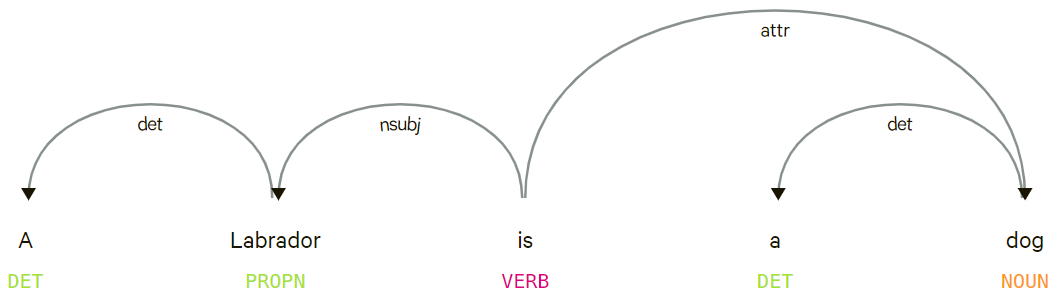
\includegraphics[width=1.\linewidth]{images/dependency_parse.png}
  \caption{Example dependency tree of a simple sentence.\index{Dependency tree}}
  \label{fig:simple_dep_tree}
\end{figure}
The dependency path can be represented as a feature according to a bespoke notation.  An edge between two words can be captured with the tuple $(lemma, pos_tag, dependency_label, direction)$ and the link between two related words expressed as a list of edges.  The link between the hyponym \textit{Labrador} and its hypernym \textit{dog} would be expressed as the sequence:
\[(Labrador, PROPN, NSUB, <), (be, VERB, ROOT, -),(dog, NOUN, ATTR, >)\]

This particular notation is used in \citep{shwartz2016path} which we found more intuitive than the older convention used in \citep{Snow2004}.  To avoid longer, potentially less precise paths, a limit on the links between nouns can be imposed.  \citep{Snow2004} opted for the shortest path consisting of a maximum of four links between any two nouns.

To avoid extreme sparsity in the path vector model, \citeauthor{Snow2004} harvested dependency paths that held for at least five different word pairs from a corpus of 6 million news article sentences \citep{Snow2004}.  Doing so they generated 69,592 distinct dependency path features.  The corpus was also used to extract training and evaluation data.  As \citeauthor{wu2012probase} did later on in \citep{wu2012probase}, \citeauthor{Snow2004} extracted hyponym-hypernym word-pairs from each sentence in their corpus.  Invoking WordNet \citep{Miller1995} as lexical resource, they split the set of pairs into known hypernymy and random words.  To consider a word-pair, both of its constituent words had to be first detected in WordNet.  An ordered word-pair $(x, y)$ would be added to the known hypernym set, if $y$ is found to be an ancestor of $x$.  Words that were not hierarchically related were consigned to the random word list.  The ratio of known hypernyms to random words was 1:50.    

The dataset was used to evaluate the quality of the mined dependency paths.  This was done by applying a simple binary classifier to each path, and predicting hypernymy if a word-pair was connected by a dependency path at least once.  This exercise supplied quantitative support for the efficacy of Hearst’s manually derived patterns, all of which were found to be highly-predictive of hypernymy.  A further four patterns were also found to be high-performing:
\begin{itemize}
    \item $Y$ like $X$;
    \item $Y$ called $X$;
    \item $X$ is a $Y$;
    \item $X$, a $Y$;
\end{itemize}

\subsection{Leveraging Classifiers to Predict Hypernymy}
Intuitively, pattern occurrence frequency should be positively correlated to hypernym detection success.  \citeauthor{Snow2004} create two \ac{VSM}s.  One is a 69,592 dimensional matrix, where each dimension represents a particular dependency path and its value is the total number of times that dependency path connected an input word-pair.  They also create a bucketed, binary vector model where each dependency path corresponds to a 14-dimension “one-hot” encoded binary vector with each dimension capturing the number of pattern occurrences on an exponential scale from 1 (single occurrence) to 8192.  Thus, every word-pair is encoded as a 974,277-dimensional, sparse vector \citep{Snow2004}.  Using the same training set employed to quantify dependency path effectiveness, they train two logistic regression classifiers using each feature vector space respectively.  A significant improvement was observed compared to a simple Hearst pattern-only baseline, which classifies hypernymy if the presence of one or more Hearst patterns is found binding the input word-pair.  Their logistic regression model trained on the bucketed, “one-hot” vectors yields a 0.3480 F1 score, a 132\% improvement over the baseline \citep{Snow2004}. 
\citeauthor{ritter2009anyway}, on the other hand, advocate analysing the word form of the pattern-matched words, prior to proposing them as viable hypernym candidates \citep{ritter2009anyway}.  In particular, words detected in the plural-form by a POS-tagger are more likely to be precise hypernyms when found in certain in patterns \citep{ritter2009anyway}.  They also examine the importance of pattern occurrence frequency in their experiments, focusing on the standard Hearst patterns.  The ambiguity of the English language makes it such that high-frequency patterns alone cannot always guarantee correct hypernyms.  The authors furnish negative hypernymy examples, despite the matching highly-occurring patterns \citep{ritter2009anyway}:
\begin{itemize}
    \item \say{…all around the world including Australia, …} $\Rightarrow$ $hypernym(Australia, world)$
    \item \say{…information about this hotel such as rates, …} $\Rightarrow$ $hypernym(rates, hotel)$
    \item \say{My dog is a bloodhound} $\Rightarrow$ $hypernym(dog, bloodhound)$
\end{itemize}

They distinguish between “left” and “right” patterns where the hyponym $X$ features to the left or right of the hypernym $Y$ in a sentence.  The first two negative examples above are instances of “right” patterns and the last an incorrect instance of a “left” pattern.  \citeauthor{ritter2009anyway} engineer a set of frequency-related features for a given a word-pair.  In addition to total distinct pattern matches, they include features that capture “left” and “right” pattern matches; the total number of times that the hyponym is related to the hypernym via the lemma \textit{be}; the percentage of matches where the hyponym is preceded by an article, determiner or quantifier; the frequency rank of the hypernym with respect to the hyponym in the pair \citep{ritter2009anyway}.   

The word-pair dataset is extracted using TextRunner \citep{banko2007open}, applied on a 117 million web page corpus, which is then validated manually.  A test data-set consisting of 953 pairs is set aside and is split into common concepts (370 pairs) and named entities (583 pairs).  The pattern frequency vector is fed into \textsc{HypernymFinder$_{SVM}$}, a \ac{SVM} classifier \citep{platt1999probabilistic} designed to improve on an earlier na\"ive rules-based classifier that excluded hypernymy in word-pairs that did not match both left and right Hearts patterns.  An \ac{SVM} classifier splits the vector space by estimating hyperplanes which maximise the distance margin between them and the closest training-set samples.    
Unlike \citeauthor{Snow2004} who used WordNet as an evaluation and comparison tool \citep{Snow2004}, \citeauthor{ritter2009anyway} merge WordNet with \textsc{HypernymFinder$_{SVM}$} to create a hybrid classifier.  
Moreover, they opt for a hypernym discovery setup, foreshadowing the SemEval Task 2018 task 9 shared task \citep{camacho2018semeval}.  They retrofit the precision and recall metrics to measure respectively the percentage of overall correct hypermys and the percentage of terms for which one correct hypernym was proposed \citep{ritter2009anyway}.  

WordNet can return high-quality hypernyms but suffers from low coverage, especially with regards to named entities.  Each test candidate was first looked up in WordNet in which 17\% and 64\% of named entities and common nouns respectively were found.  Given some bounded vocabulary (details of which are elusive in their paper), the hybrid classifier outputs the five words it considers most likely to be hypernyms of the test words missing in WordNet.  In this manner, \citeauthor{ritter2009anyway} boosted the WordNet baseline for named entities and, to a lesser extent, common nouns.  Recall/precision increased from 0.17/1.0 to 0.32/0.9 and from 0.64/1.0 to 0.7/0.9 for named entities and common nouns respectively \citep{ritter2009anyway}.  Precision suffers with increased recall since the classifier’s output cannot be of the gold-standard level maintained in WordNet.

\subsection{Identifying Co-hyponyms to Increase Recall}
\citep{Snow2004} and \citep{ritter2009anyway} both acknowledge the limitation of Hearst patterns \citep{hearst1992automatic}.  Most hypernyms simply do not feature in the same sentence with their hyponyms \citep{Snow2004, ritter2009anyway}.  They hypothesise about extending the confines of the sentence for an “orphan” hyponym (i.e. no companion hypernym was found for it in a sentence) by finding co-hyponyms with known hypernyms.  If $(x_i, x_j)$ are two coordinate nouns and $hypernym(x_i, NA)$, $hypernym(x_j, y)$ then we can deduce $hypernym(x_i, y)$.

\citeauthor{Snow2004} experiment with various techniques including: building a distributional similarity vector space model; resorting to WordNet to find co-hyponyms for supported terms; and using high frequency conjunction dependency patterns.  Using the distributional similarity vector space the words can be scored for co-hyponym similarity using the symmetric cosine measure.  A linear combination of the probabilities calculated by the hypernym-only classifier and coordinate classifier increased the $F1$ score by 20\% compared to a hypernym-only classifier on a hand-labelled dataset ($F1$ of 0.3268 and 0.2714 respectively) \citep{Snow2004}.

On the other hand, \citeauthor{ritter2009anyway} were inspired by \textsc{Realm} \citep{downey2007sparse}, which uses \ac{HMM}s to perform type checking in an Information Extraction system, especially if the term in question is sparsely represented in vector space.  In \ac{HMM}s, a hidden stochastic process can only be glimpsed at through another stochastic process that produces a sequence of observations.  No information is known about the model's state but we can assume that there exists some model that can generate the data we're able to observe \citep{rabiner1989tutorial}.  For instance, \textit{Pickerington, Ohio} and \textit{Chicago, Illinois} are both cities but the former will be mentioned much less frequently in a balanced corpus.  Using traditional distributional similarity measures, it is unlikely that \textit{Pickerington} and \textit{Chicago} will be deemed similar since the contexts in which they appear are different.  However given an \ac{HMM} with $n$ hidden states that models the corpus, it is possible that $., Ohio$ and $., Illinois$ were generated by the same hidden states since both terms represent US States \citep{downey2007sparse} in \citep{ritter2009anyway}.

\citeauthor{ritter2009anyway} applied the same concept to finding terms similar to a given hyponym.  To do so, a word is represented by the distribution of the hidden states’ probability of the term being generated by the \ac{HMM} model.  Thus, given an \ac{HMM} model with $n$ states, an $n$-dimensional vector representation is returned.  Similar words to a given term were found by applying a similarity metric on the \ac{HMM}-based feature vector.  The final incarnation of the authors' hypernym finder, is a linear combination of the probability calculated by the \textsc{HypernymFinder$_{SVM}$} classifier and the probability that a given term $x$ has a coordinate word which is a hyponym of the candidate hypernym $y$. Since word similarity alone is tenuous evidence for such words sharing a hypernym, the \ac{HMM} classifier predicts hypernymy in a $(x, y)$ word-pair only if $x'$ exceeds a similarity threshold with $x$, and $x'$ is hyponym of $y$ \citep{ritter2009anyway}.

\subsection{Encoding Dependency Paths with an LSTM}
We have seen that using dependency paths as features can lead to a highly-dimensional vector space.  In one study we have examined, almost 70,000 distinct dependency paths were extracted from a corpus.  Vectors will be sparse since a particular word-pair will only activate a small number of dependency paths.  To improve dependency path representation, \citeauthor{shwartz2016path} trained a \ac{LSTM} \citep{hochreiter1997long} encoder to learn path vectors that are optimised towards detecting hypernymy \citep{shwartz2016path}.  The path vectors are fed into a classifier which predicts whether the dependency pattern feature captures the hypernymy relationship in a given word-pair.  The model is referred to as \textbf{HypeNET} \citep{shwartz2016path}.

The LSTM belong to a family of neural models known as \ac{RNN}s.  Contrary to regular densely-connected networks which require an entire sequence to be presented at once, \ac{RNN}s can be fed the input, one time-step at a time \citep{chollet2017deep}.  A limitation of \ac{RNN}s is their difficulty to recognise signals that come from distant points in a past sequence which does not make them the ideal choice to learn long-term dependencies.  The \ac{LSTM} overcomes this problem because it is a type of recurrent neural network with the ability to learn long-term dependencies.  By having access to the previous time-steps, it is able to build temporal patterns.  Through the use of a special gate composed of a dot product operator and activation function, it can selectively “forget” irrelevant signals whilst retaining information that is more important at the current time-step \citep{chollet2017deep}.  

The motivation behind using the \ac{LSTM} approach is to generalise the lexical-semantic relation between terms that holds in a multitude of contexts.  Prior to feeding them to the \ac{LSTM}, each word-pair is represented by a sequence of dependency paths in which the words co-occur in the corpus.  To be considered, a word-pair needs to co-occur in the corpus and be represented by at least two unique dependency paths.  The path is represented by a list of edge vectors with each edge made up of the concatenation of the embeddings of the lemma, \ac{POS} tag, dependency label and direction.  The dimensionality of the embeddings vary: \citeauthor{shwartz2016path} use 50, 4, 5, and 1 dimension for each respective component \citep{shwartz2016path} although this is not set in stone.  Hyper-parameter tuning on a validation set can help determine the best network configuration.  The \ac{LSTM} should learn which dependency path sequences are predictive of hypernymy while conveniently forgetting those which have no consequence on the semantic relationship \citep{shwartz2016path}.

The weighted-average of the encoded dependency path vectors is computed prior to feeding it to a softmax classifier, trained to minimise cross entropy loss.  The softmax classifier assigns a probability for both the hypernymy and non-hypernymy target labels, which sum up to 1.

\citeauthor{shwartz2016path} compare their novel approach to \citeauthor{Snow2004}'s model \citep{Snow2004} we discussed in section \ref{Learning Patterns Automatically}. The authors train a logistic regression classifier on the 100,000 most information paths chosen using chi-squared feature selection.  On a random data split, the sparse model returns a precision of 0.843 compared to HypeNET’s 0.811 but the latter scores 0.716 recall, a 58\% improvement over \citeauthor{Snow2004}'s model.    

%%Għidli ma’ min tagħmilha, u ngħidlek x’int